%%%%%%%%%%%%%%%%%%%%%%%%%%%%%%%%%%%%%%%%%
% Journal Article
% LaTeX Template
% Version 1.3 (9/9/13)
%
% This template has been downloaded from:
% http://www.LaTeXTemplates.com
%
% Original author:
% Frits Wenneker (http://www.howtotex.com)
%
% License:
% CC BY-NC-SA 3.0 (http://creativecommons.org/licenses/by-nc-sa/3.0/)
%
%%%%%%%%%%%%%%%%%%%%%%%%%%%%%%%%%%%%%%%%%

%----------------------------------------------------------------------------------------
%	PACKAGES AND OTHER DOCUMENT CONFIGURATIONS
%----------------------------------------------------------------------------------------

\documentclass[twoside]{article}

\usepackage{lipsum} % Package to generate dummy text throughout this template

\usepackage[sc]{mathpazo} % Use the Palatino font
\usepackage[T1]{fontenc} % Use 8-bit encoding that has 256 glyphs
\linespread{1.05} % Line spacing - Palatino needs more space between lines
\usepackage{microtype} % Slightly tweak font spacing for aesthetics

\usepackage[hmarginratio=1:1,top=32mm,columnsep=20pt]{geometry} % Document margins
\usepackage{multicol} % Used for the two-column layout of the document
\usepackage[hang, small,labelfont=bf,up,textfont=it,up]{caption} % Custom captions under/above floats in tables or figures
\usepackage{booktabs} % Horizontal rules in tables
\usepackage{float} % Required for tables and figures in the multi-column environment - they need to be placed in specific locations with the [H] (e.g. \begin{table}[H])
\usepackage{hyperref} % For hyperlinks in the PDF

\usepackage{lettrine} % The lettrine is the first enlarged letter at the beginning of the text
\usepackage{paralist} % Used for the compactitem environment which makes bullet points with less space between them

\usepackage{abstract} % Allows abstract customization
\renewcommand{\abstractnamefont}{\normalfont\bfseries} % Set the "Abstract" text to bold
\renewcommand{\abstracttextfont}{\normalfont\small\itshape} % Set the abstract itself to small italic text

\usepackage{titlesec} % Allows customization of titles
\renewcommand\thesection{\Roman{section}} % Roman numerals for the sections
\renewcommand\thesubsection{\Roman{subsection}} % Roman numerals for subsections
\titleformat{\section}[block]{\large\scshape\centering}{\thesection.}{1em}{} % Change the look of the section titles
\titleformat{\subsection}[block]{\large}{\thesubsection.}{1em}{} % Change the look of the section titles

\usepackage{fancyhdr} % Headers and footers
\pagestyle{fancy} % All pages have headers and footers
\fancyhead{} % Blank out the default header
\fancyfoot{} % Blank out the default footer
\fancyhead[C]{} % Custom header text
\fancyfoot[RO,LE]{\thepage} % Custom footer text

\usepackage{graphicx}

%----------------------------------------------------------------------------------------
%	TITLE SECTION
%----------------------------------------------------------------------------------------

\title{\vspace{-15mm}\fontsize{24pt}{10pt}\selectfont\textbf{Evaluation of Classification Algorithms for Machine Learning in Advertising Technology}} % Article title

\author{
\large
\textsc{Vangie Shue}\\[2mm] % Your name
\normalsize New York University \\ % Your institution
\normalsize \href{mailto:vangieshue@gmail.com}{vangieshue@gmail.com} % Your email address
\vspace{-5mm}
}
\date{}

%----------------------------------------------------------------------------------------

\begin{document}

\maketitle % Insert title

\thispagestyle{fancy} % All pages have headers and footers

%----------------------------------------------------------------------------------------
%	ABSTRACT
%----------------------------------------------------------------------------------------

\begin{abstract}

\noindent
This project investigates the application of machine learning in advertising technology, a rapidly growing field. In order to utilize machine learning in advertising technology however, a balance must be found between accuracy and efficiency. As such, this project will provide a preliminary comparison of several algorithms on the basis of how long they take to fit a large amount of data and how accurate their resulting model is. The algorithms will be used to tackle a binary classification problem, specifically: determining hispanic users from the audience in order to target them for advertising campaigns? For our study, we limited our analysis to the following algorithms: Naive Bayes, Gradient Boosting, Logistic Regression, and Support Vector Machines--all of which have an associated library available in R. From our results, we found the generalized linear model and gradient boosted model implementations to have the best performance for our use case. 
\textbf{Keywords--analytics, online advertising, classification, machine learning}

\end{abstract}

%----------------------------------------------------------------------------------------
%	ARTICLE CONTENTS
%----------------------------------------------------------------------------------------

\begin{multicols}{2} % Two-column layout throughout the main article text

\section{Introduction}

\lettrine[nindent=0em,lines=3]{O} nline advertising has undergone sweeping development thanks to fairly recent but rapid innovation and advancement of tools allowing advertisers to automate the management, evaluation, and analysis of their display advertising campaigns. Services like Nielsen Online Campaign Ratings for example, provide demand-side clients, the advertisers, with the ability to determine whether their ads are reaching particular user populations that are more likely to be interested in their products. On the supply-side, companies like Mediamath offer management applications that allow the publishers more control over how their ads are distributed such as by setting daily impression caps and black- or white-listing particular websites. With these improvements to help streamline campaign management, advertisers can now focus on solving more abstract questions and develop more fine-tuned targeting strategies, thus improving the return on their investments\cite{12}.

There is a great opportunity to utilize machine learning in identifying pertinent users so that more relevant ads can be targeted to them. Publishers can track how their users typically navigate their sites through tracking pixels and cookies\cite{13}. With services like Demdex, a data management platform, they can create traits to define their users. Multiple traits can be further clustered into segments. When publishers receive their impression reports, they are able to see which traits/segments a particular cookie (or "user") satisfies. In machine learning, traits and segments would be analogous to features, while each cookie can act as a data point. As such, a medium-sized company, with nearly four million cookies accessing their sites per day, quickly aggregates a tremendous amount of data.

CafeMom is an online community for moms to come together to exchange advice and support on topics like pregnancy, health, etc. One of their flagship services is MamasLatinas, a site geared towards providing a more relevant community for Hispanic moms. Many advertisers commission CafeMom to help bring their products to Hispanic moms, leading CafeMom to need to develop a reliable model to identify Hispanic women so that they can target these users in both on- and off-site advertisements. But even a simple problem like binary classification can be modeled in many ways in machine learning. This project therefore seeks to provide a preliminary evaluation of the typical learning algorithms that could solve this problem: Naive Bayes, Gradient Boosting, Logistic Regression, and Support Vector Machines. Advertising data is big in scale not only because there are so many online users, but also because it contains a tremendous number of features. As such, the study will need to compare these algorithms both in terms of how quickly they can model the data and how accurately their model predicts on test data.

\subsection{Classifying Rare Events}
While CafeMom may be able to obtain a significant amount of information on Hispanic users through MamasLatinas, they are interested in seeing how these users navigate on other sites in order for them to be able to identify Hispanic moms on affiliated sites. In addition, when sampling, we must be careful not to select on X differently for the two samples \cite{1}. Therefore, our project only guarantees a Hispanic user based on their User Agent language. The complement is only considered to be users who use English for their User Agent. As such, in the grand schemes of all their users, Hispanic moms actually constitute only around 2\% of their known population of data. Identifying a Hispanic mom is therefore actually a fairly rare event.

According to King and Zeng, rare events tend to be difficult to explain and predict\cite{1}. Either logistic regression algorithms will sharply underestimate these events or data collection strategies are grossly inefficient\cite{1}. In addition, the authors identified that rare events are actually more statistically informative than "zeros"\cite{1}. King and Zeng determined that they could achieve better results by sampling all available events and only a tiny fraction of non-events. This method would also have the added benefit of being more efficient since you would not have to model over [as] tremendous amounts of data in order to get a sufficient number of events while maintaining the event probability.

On the other hand, Paul Allison responded with some critique to the study\cite{2}. He believed that the problem was not actually the "rarity" of the events but the actual \textbf{number} of events was too small, and therefore led to small-sample bias in logistic models. By example, Allison believed that as long as the sample of rare events was large enough (ex. 2000 events), you could still model on the original sample size (ex. 100,000 cases). In addition, Paul Allison suggested the use of penalized likelihood, or the Firth method, to model data with rare events\cite{2}. However, since modeling with enough data to reduce the small-sample bias would drastically increase the execution time, this project will utilize the method offered by King and Zeng. However, we will do a brief comparison of the weighted event method with a non-weighted sample to provide a glimpse as to whether the results would be significantly different.

\subsection{Classification Algorithms}
In an attempt to cover the breadth of learning algorithms for binary classification, we have chosen to evaluate the following algorithms: Naive Bayes, Support Vector Machine, Gradient Boosted Model, and Logistic Regression. All have implementations available in R, which was therefore our language of choice for this study. We will use prediction rate as a measure of goodness of fit, but also look at the rate of false-postives and false-negatives to get an even clearer idea of how the model predicts on data.

\subsubsection{Naive Bayes}
Naive Bayes is a supervised learning algorithm based on applying the Bayes' theorem with the "naive" assumption of independence between every pair of features. As such, we hypothesize that the modeling time would be on the shorter end of the spectrum, but could suffer in terms of prediction quality. The decision rule for Bernoulli Naive Bayes is based on the following\cite{15}:
\[ P(x_i | y) = P(i | y)*x_i + (1 - P(i | y))(1 - x_i) \]
It explicitly penalizes the non-occurrence of a feature\cite{15}. This study will use the \texttt{naiveBayes()} in \textbf{e1071} as is is the more popular of the two available \texttt{R} libraries that support Naive Bayes modeling\cite{22}.

\subsubsection{Random Forest}
Random Forest was initially considered for this study as it is a distinctive algorithm for classification. Random forest tends to perform well, but unfortunately, they suffer heavily with sparse data where bagging and splitting is wasted on non-events. In addition, they are very memory intensive due to the process of growing many classification trees\cite{19}. Even with \textbf{bigrf}, a random forest library in R geared towards big matrices\cite{20}, a test on the "smallest" sample of training data caused the machine to abort, so random forest was decidedly not used for this research.

\subsubsection{Support Vector Machines}
Support Vector Machines are among the most popular and efficient classification methods used. Fundamentally, SVMs try to find the hyperplane with the maximum margin, or the optimal canonical hyperplane, by identifying the weight vector and bias that yield the maximum margin of all possible separating hyperplanes\cite{23}. Currently, four \texttt{R} packages offer SVM modeling. A paper by Karatzoglou, Meyer, and Hornik compared these packages and concluded that \texttt{ksvm()} in the \textbf{kernlab} was the most flexible SVM implementation as it allowed for user-defined kernels. On the other hand, \texttt{svm()} in the \textbf{e1071} package is a 'robust interface to the award-winning \textbf{libsvm} SVM library\cite{21}. As such, we chose to use \textbf{e1071}'s \texttt{svm()} for this study as it was meant to cover more breadth than depth and therefore would not be exploring tuning parameters too intimately.
\[ K(x_i, x_j) = (x_i^T)x_j + 1 \]

\subsubsection{Gradient Boosted Model}
Gradient boosting model involves the application of boosting to regression trees. A gradient boosted model is initially composed of very simple trees and successive trees are added to predict the residuals of the preceding tree\cite{27}. Gradient boosted model, or generalized boosted model as it is called in the \textbf{gbm} package available in R, is considered to have several advantages over logistic regression: robustness to outliers, predicting on missing data, handling of unequal class sizes and unbalanced predictor variables, as well as tending to have greater predictive ability\cite{7}. Of course, a model is not without drawbacks, and may suffer from overfitting especially if the number of ending nodes is too small or number of trees is too large\cite{7}. Thus, cross validation is highly recommended if gradient boosted model is the algorithm of choice. However, this study will observe how well the modeled works without the additional tuning via cross validation.

\subsubsection{Logistic Regression}
It shouldn't come as a surprise that logistic regression was included in our survey algorithms. Logistic regression is actually a model for classification, and typically binary classification, contrary to what its name might suggest\cite{30}. It is based on the logistic function, \(F(t)\) where \texttt{t} is a linear function of an explanatory variable \texttt{x}, which outputs a binary value given an input that can range from positive to negative infinity\cite{10}:
\[ F(t) = 1/(1 + e^{-t}) \]
Logistic regression is in fact part of a broader family of models, known as generalized linear models. Logistic regression is the subset where the response is binomial\cite{32}. This study will actually be investigating the logistic regression implementation in the \textbf{glmnet} package as it is intended for large datasets. \texttt{glmnet} fits a generalized linear model via penalized maximum likelihood\cite{4}. It boasts a robust implementation that can handle very large sparse matrices\cite{6}, a particular data structure in \texttt{R}. As such, using \textbf{glmnet} would enable training on data even a hundred times larger than what the other methods studied here can handle. Of course, training on such large data will still be very slow and memory-intensive even with this particular package.

%------------------------------------------------

\section{Design}

The data used in this study was provided by CafeMom. The raw data is provided via hourly logs from Adobe Demdex. The logs are tab-delimited with a field for unique user ID (uuid) and a comma-delimited array of IDs referring to the traits that that user has satisfied. The data is read as a hive table and partitioned into hispanic and non-hispanic based on the user's User Agent trait. A hispanic user is assumed to have either trait 780664 or 920203 (e.g. their User Agent language is Spanish) while a non-hispanic user is assumed to have either trait 783538 or 920206 (their User Agent language is English). This is to ensure that our data is complementary and does not accidentally bias towards either group.

\begin{verbatim}
insert overwrite table segment_hispanic 
partition(class)
select uuid, max(case when datatype = 4 
and (array_contains(varints,780664) 
or array_contains(varints,920203))
then 1 else 0 end ) class
from user_attribs2
where (datatype = 4 and 
(array_contains(varints,780664) 
or array_contains(varints,783538) 
or array_contains(varints,920203) 
or array_contains(varints,920206)))
group by uuid;
\end{verbatim}

In total, the data had 80,324,851 total uuids with 1,698,878 uuids attributed to hispanic users. The percent of hispanic users in our population is therefore approximately 5\%. In accordance to the King and Zeng paper, which advised that the non-events be no more than 2- to 5-times the events, we weighted the hispanic users by selecting all the hispanic uuids and only 10\% of the non-events.

\begin{verbatim}
insert overwrite table segment_hispanic2
partition(class)
select * from ( 
select * from segment_hispanic 
where class = 1 
union all 
select * from segment_hispanic 
tablesample(bucket 1 out of 10)
) s;
\end{verbatim}

The table segment\_hispanic2 consequently had 9,733,751 total uuids with around 19\% being hispanic uuids. The data was then processed with R such that the array of traits over all the UUIDs were exploded into separate columns, constituting the feature space. The matrix had 2,105,480 features. After sampling 1.5\% rows from the matrix so that we could limit how long the modeling would take, we removed all features  that were positive for fewer than 50 UUIDs. This data subset now had 142,433 UUIDs (rows) and 10,128 features (columns). The data was then further partitioned such to set aside approximately 1\% of the data to use as test/validation data.

In order to compare the algorithms on their model-fitting speed, we fitted the model using the original data, 0.5\% (approx. 70,000 rows), and 0.25\% (approx. 35,000 rows) of the data. We then used the first model (based on "all" the data) to determine how long it took to predict on 100, 250, 500, and 1000 rows of test data. Finally, we compared how much the accuracy improved by testing the three models on five samples ot 500 rows of test data. If time permitted, we tested several tuning parameters to see if it would significantly improve the performance of the algorithm in either speed or accuracy.

\subsection{Naive Bayes}
Fitting and predicting data with \texttt{naiveBayes} in R is very simple\cite{16}. By default, laplace smoothing is set to 0\cite{16}. Increasing the smoothing would likely decrease the modeling time but at the risk of underfitting. Since our data is already very sparse, we used the default laplace smoothing. Perhaps for the same reason, varying the threshold for the prediction did not vary the outcome.
\begin{verbatim}
library(e1071)
system.time(fitnb<-naiveBayes(
                x=datatrain
                , y=as.factor(ytrain)
                , laplace=0))
system.time(prednb<-predict(
            object=fitnb
            , newdata=datatest
            , type="class"
            , threshold=0.001))
\end{verbatim}

\subsection{Support Vector Machines}
The package \textbf{e1071} also contains \texttt{svm()}. Its implementation is similar to Naive Bayes\cite{24}. We use C-classification, also known as Classification SVM Type 1\cite{26}. We chose to use the linear kernel as it is the preferred kernel when dealing with large sparse data vectors\cite{23}. The parameters cost, class.weights, tolerance, epsilon, and shrinkage were kept at their default values\cite{24} to minimize over-tuning.
\begin{verbatim}
library(e1071)
system.time(fitsvm<-svm(
                x=datatrain
                , y=as.factor(ytrain)
                , scale=FALSE
                , type="C-classification"
                , kernel="linear"
                , probability=TRUE))
system.time(predsvm<-predict(
              object=fitsvm
              , newdata=datatest
              , probability=TRUE))
\end{verbatim}

\subsection{Gradient Boosted Model}
The \textbf{gbm} package in R allows control over several parameters. We set the distribution to "bernoulli" since this is a binary classification problem. The number of trees to fit dictates the number of iterations and basis functions in the additive expansion\cite{29}. Best practice would be to set the number of trees to a large number and prune it back afterwards, but to limit the modelling time, we will fit with 100 trees. The shrinkage is the step size or learning rate, which we chose to be 0.1. A smaller step would take longer to model although it could yield better performance. The interaction depth limits the maximum depth of variable interactions, where 1 would imply an additive model and 2 would imply up to two-way interaction, and so forth. Cross-validation can be used to determine the interaction depth. While increasing the interaction depth may produce a closer model, it will also increase the fitting time substantially. The \texttt{n.minobsinnode} parameter sets the minimum number of observations for a terminal node. Decreasing this value increases in-sample fit but therefore risks overfitting. We did perform a simple tuning test to identify the effect of the interaction depth by observing the time to fit if the interaction depth was 1 or 3 (compared to a depth of 2 which we used for our comparison with the other algorithms).
\begin{verbatim}
library(gbm)
system.time(fitgbm<-gbm.fit(
            x=datatrain[train0,]
            , y=ytrain[train0]
            , distribution="bernoulli"
            , n.trees = 100
            , shrinkage = 1
            , interaction.depth = 2
            , n.minobsinnode = 10
            , keep.data = FALSE
            , verbose = FALSE))
system.time(newtrees<-gbm.perf(
            fitgbm, method="cv"))
system.time(predgbm<-predict.gbm(
            object=fitgbm
            , newdata=datatest
            , n.trees=newtrees
            , type="response"))
\end{verbatim}

\subsection{Logistic Regression}
We used \texttt{glmnet} to generate our logistic regression models. Its usage is quite straightforward in R. Besides setting the family parameter to "binomial", all other parameters were kept at default values. This meant that the features were equally weighted, there was no offset, the elasticnet mixing parameter alpha was 1 (LASSO penalty), and the number of lambda values was 100\cite{4}. The LASSO penalty, or least absolute shrinkage and selection operator, penalizes the absolute size of the regression coefficients. The remaining parameters were undefined as they did not apply to the binomial problem.
\begin{verbatim}
library(gbm)
system.time(fitglm<-glmnet(
            x=datatrain[train0,]
            , y=ytrain[train0]
            , family="binomial"))
system.time(predglm<-predict(
            object=fitglm
            , newx=datatest
            , type="response"))
\end{verbatim}

%------------------------------------------------

\section{Results}

\subsection{Naive Bayes}

From Table 1 we find that the modelling time increased almost linearly with restpect to the size of the training data. This is expected since Naive Bayes does not consider feature interactions, so it can fit the classifier in \texttt{O(m*n)} time, where \texttt{m} is the number of training examples and \texttt{n} is the number of features. Figure 2 shows the nearly linear relationship between the size of the test data and how long it took to produce to the predictions. Finally, Figure 3 demonstrates the correlation between the accuracy of the predictions and the amount of data used to train the model. In addition, the blue line indicates the change in percent of false-positives, while the red line indicates the percent change in false-negatives. The accuracy appears to increase almost linearly and mostly due to the decrease in false-negatives. The average accuracy of the Naive Bayes model was 80.6\%.

\begin{table}[H]
\caption{Naive Bayes fitting times}
\centering
\begin{tabular}{llr}
\toprule
m (\#) & Time (s) \\
\midrule
$35000$ & $82.248$ \\
$70000$ & $167.030$ \\
$142433$ & $294.883$ \\
\bottomrule
\end{tabular}
\end{table}

\begin{table}[H]
\caption{Naive Bayes predicting times}
\centering
\begin{tabular}{llr}
\toprule
m (\#) & Time (s) \\
\midrule
$100$ & $33.053$ \\
$250$ & $82.095$ \\
$500$ & $168.915$ \\
$1000$ & $335.145$ \\
\bottomrule
\end{tabular}
\end{table}

\begin{figure}[H]
 \caption{Naive Bayes performance (black: accuracy, blue: false-positve, red: false-negative)}
  \centering
    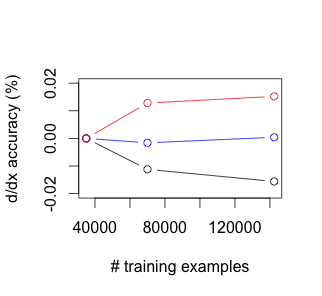
\includegraphics[width=8cm]{../data/nb_acc}
\end{figure}

\subsection{Support Vector Machines}
From Figure 1, we see that the modelling time begins to increase exponentially as the number of training examples increases. At 140,000 plus data points, the modelling took more than 1.5 hours. In Figure 2, predicting time was nearly linear with respect to the number of test cases and fairly quick. Figure 3 shows small decrease in the accuracy, a small decrease in the false-negatives percent, and an increase in false-positives. The accuracy of the SVM predictions averaged at 89.1\%.

\begin{table}[H]
\caption{SVM fitting times}
\centering
\begin{tabular}{llr}
\toprule
m (\#) & Time (s) \\
\midrule
$35000$ & $436.036$ \\
$70000$ & $1531.416$ \\
$142433$ & $6470.774$ \\
\bottomrule
\end{tabular}
\end{table}

\begin{table}[H]
\caption{SVM predicting times}
\centering
\begin{tabular}{llr}
\toprule
m (\#) & Time (s) \\
\midrule
$100$ & $6.115$ \\
$250$ & $7.448$ \\
$500$ & $9.808$ \\
$1000$ & $14.865$ \\
\bottomrule
\end{tabular}
\end{table}

\begin{figure}[H]
 \caption{SVM performance (black: accuracy, blue: false-positve, red: false-negative)}
  \centering
    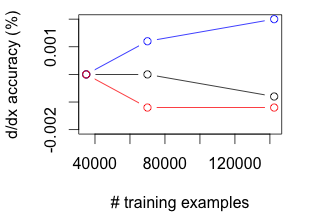
\includegraphics[width=8cm]{../data/svm_acc}
\end{figure}

\subsection{Gradient Boosted Model}
Gradient boosted models also take a significant amount of time to generate, but at least their times appear to only increase linearly as opposed to exponentially. Fitting slightly less than 150,000 data points took a little over 1 hour. However, as a tradeoff, the predicting times are extremely fast--only our largest test sample, it finished predicting in less than 1 second. Unlike SVMs and Naive Bayes, the accuracy did not appear to improve significantly when the model was fitted using more data. The accuracy averaged at around 89.4\%. 

Varying the interaction depth did indeed significantly affect the modelling time. The default we used of 2 took around 17 minutes to model the small training dataset. When the interaction depth was set to 1, the time decreased to 9.5 minutes, nearly half the time. When the interaction depth was 3, the modelling took almost 25 minutes. The difference is significant but could be acceptable for our use case. An interaction depth of 2 actually appeared to predict on our test data best. At different depths, the accuracy varied from from 89.4\% at a depth of 1, to 89.8\% at a depth of 2, and 89.6\% at a depth of 3.

\begin{table}[H]
\caption{GBM fitting times}
\centering
\begin{tabular}{llr}
\toprule
m (\#) & Time (s) \\
\midrule
$35000$ & $1004.997$ \\
$70000$ & $2006.688$ \\
$142433$ & $4103.233$ \\
\bottomrule
\end{tabular}
\end{table}

\begin{table}[H]
\caption{GBM predicting times}
\centering
\begin{tabular}{llr}
\toprule
m (\#) & Time (s) \\
\midrule
$100$ & $0.078$ \\
$250$ & $0.133$ \\
$500$ & $0.254$ \\
$1000$ & $0.464$ \\
\bottomrule
\end{tabular}
\end{table}

\begin{figure}[H]
 \caption{GBM performance (black: accuracy, blue: false-positve, red: false-negative)}
  \centering
    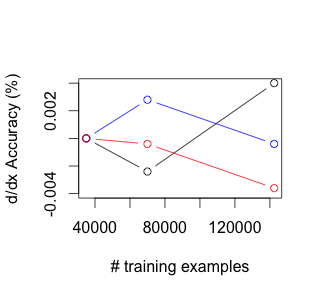
\includegraphics[width=8cm]{../data/gbm_acc}
\end{figure}

\subsection{Logistic Regression}
The fitting time for \textbf{glm} also increase significantly with additional training examples in a seemingly exponential fashion. The predicting time however, is almost half that of the general boosted model.

\begin{table}[H]
\caption{GLM fitting times}
\centering
\begin{tabular}{llr}
\toprule
m (\#) & Time (s) \\
\midrule
$35000$ & $951.781$ \\
$70000$ & $2158.661$ \\
$142433$ & $6102.381$ \\
\bottomrule
\end{tabular}
\end{table}

\begin{table}[H]
\caption{GLM predicting times}
\centering
\begin{tabular}{llr}
\toprule
m (\#) & Time (s) \\
\midrule
$100$ & $0.034$ \\
$250$ & $0.076$ \\
$500$ & $0.161$ \\
$1000$ & $0.274$ \\
\bottomrule
\end{tabular}
\end{table}

\begin{figure}[H]
 \caption{GLM performance (black: accuracy, blue: false-positve, red: false-negative)}
  \centering
    \includegraphics[width=8cm]{../data/glm_fit}
\end{figure}

\subsection{Comparison}

\begin{figure}[H]
 \caption{Fitting times for the four algorithms (black: Naive Bayes, blue: SVM, red: GBM, purple: GLM)}
  \centering
    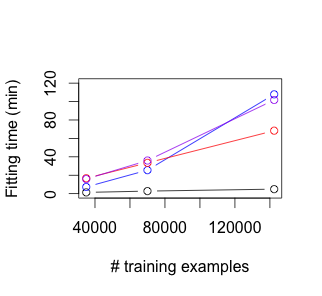
\includegraphics[width=8cm]{../data/all_fit}
\end{figure}

In Figure 5, the fitting times for the four algorithms were overlayed to provide a better visual comparison (naive bayes = black, SVMs in blue, GBM in red, and GLM in purple). In Figure 14, their predicting times are compared. And finally, in Figure 15, we compare their accuracies.

\begin{figure}[H]
 \caption{Fitting times for the four algorithms (black: Naive Bayes, blue: SVM, red: GBM, purple: GLM)}
  \centering
    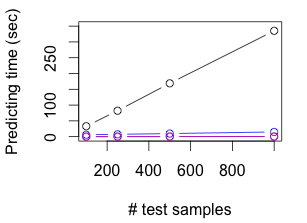
\includegraphics[width=8cm]{../data/all_pred}
\end{figure}

%------------------------------------------------

\section{Discussion}

In this study, we performed a comparison of several machine learning algorithms in order to determine which would be most appropriate for our use case. Advertising technology problems often involves tremendous amounts of data with similarly large feature space. We also need to consider the predicting times because all test data will need to be scored against the model. In addition, models need to be generated regularly to adapt to new data and changes in user behavior. This creates a very unique problem where both time and accuracy need to be balanced.

Our results suggest that in their basic implementations, Naive Bayes has demonstrated the worst behavior. Though it can generate a model in linear time, the accuracy was very poor compared to the other algorithms. In addition, predicting on test data took longer compared to the other algorithms. This will eventually be problematic given that huge test samples will need to be scored with the model. Support Vector Machines demonstrated good accuracy, but their fitting time was problematic, increasing exponentially given additional data. Their predicting time was decent, but an order of magnitude slower than that of the gradient boosted model and generalized linear model. Gradient Boosted Model and Generalized Linear Model were fairly similar and equally promising in their performance. Both predicted quickly, at less than a second for more than 100,000 test cases, and their accuracies were both around 90\%. The generalized linear model however appears to increase more sharply in fitting time as the training sample gets larger, though it has the advantage of being able to read larger datasets than \textbf{gbm}.

Our results should not be interpreted as a standard comparison of these algorithms. Since most algorithms, and their implementations in R, allow for the tuning of parameters (such as decreasing the learning rate), without a doubt, the performance of these algorithms could be improved to yield more precise results. We did perform some preliminary tuning tests to demonstrate performance-changes based on tuning parameters. For example, increasing interaction depth did increased fitting time for \textbf{gbm} but does not appear to improve the predicting ability of the model. This project mainly seeks to provide a general approach for evaluating classification models, particularly in the context of our use case in display advertising.

This study also confirms Zeng and King's methodology of training with rare event data. Though hispanic users are only 2\% of our raw training data, we oversampled them to achieve a 20\% distribution. The models were still able to achieve a 90\% accuracy in their predictions on non-biased sample. This confirms that we can reliably utilize a weighted dataset of rare events to perform our training, enabling us to model efficiently yet remaining equally if not more accurate.

While the results are encouraging, further exploration of machine learning tools is needed especially for processing large amounts of data with a similarly immense feature space. Apache Mahout is a very promising option as the project is aimed towards scalable machine learning and may allow us to test additional algorithms like random forest\cite{18}. Alternatively, using SparkR would allow for integration of R's diverse offering of machine learning tools and the parallel processing power of Spark\cite{8}. However, these technologies are still very new and undergoing significant amounts of development. Furthermore, they are also limited in their available documentation and resources. Nonetheless, moving forward we expect to see much advancement in machine learning tools to solve problems in advertising technology.

%------------------------------------------------

\section{Acknowledgements}

I would like to thank Patrick McCann at Cafemom for providing guidance for this project as well as allowing the use of Cafemom's advertising data to perform this research. In addition, I would like to thank Professor Mohri, who has imparted invaluable knowledge on machine learning algorithms in Foundations of Machine Learning (CSCI-GA. 2566-001).

%----------------------------------------------------------------------------------------
%	REFERENCE LIST
%----------------------------------------------------------------------------------------

\begin{thebibliography}{99} % Bibliography - this is intentionally simple in this template

\bibitem{12} Connolly, M (2014). What is next for the world of advertising technology? The Wall. http://wallblog.co.uk/2014/02/12/what-is-next-for-the-world-of-advertising-technology/
\bibitem{13} (2014) Display Advertising Fundamentals: the Key Players. http://www.grovo.com/display-advertising-fundamentals/the-key-players
\bibitem{1} King, G. and Zeng, L. (2001). Logistic Regression in Rare Events Data. Society for Political Methodology, WV006-01.
\bibitem{2} Allison, P (2012). Logistic Regression for Rare Events. Statistical Horizons: http://www.statisticalhorizons.com/logistic-regression-for-rare-events
\bibitem{15} (2014). 1.7. Naive Bayes. scikit: learn. http://scikit-learn.org/stable/modules/naive\_bayes.html
\bibitem{22} (2014). Data Mining Algorithms in R/Classification/Naive Bayes. WikiBooks: http://en.wikibooks.org/wiki/Data\_Mining\_Algorithms\_In\_R/Classification/Na\%C3\%AFve\_Bayes
\bibitem{19} Breiman, L. and Cutler, A. Random Forests. https://www.stat.berkeley.edu/\~breiman/RandomForests/cc\_home.htm
\bibitem{20} Lim, A (2014). Package 'bigrf'. CRAN R-Project: http://cran.r-project.org/web/packages/bigrf/bigrf.pdf
\bibitem{23} (2014). Data Mining Algorithms in R/Classification/SVM. WikiBooks: http://en.wikibooks.org/wiki/Data\_Mining\_Algorithms\_In\_R/Classification/SVM
\bibitem{21} Karatzoglou, A., Meyer, D., and Hornik, K. (2006). Support Vector Machines in R. Journal of Statistical Software. Apr 2006: 15, 9. http://www.jstatsoft.org/v15/i09/paper
\bibitem{27} (2014). Introduction to Boosting Trees for Regression and Classification. StatSoft. http://www.statsoft.com/Textbook/Boosting-Trees-Regression-Classification
\bibitem{7} Campbell, W. (2014). Using a GBM for Classification in R. http://vimeo.com/71992876
\bibitem{30} Christopher M. Bishop (2006). Pattern Recognition and Machine Learning. Springer. p. 205.
\bibitem{10} Bifet, A., Kirkby, R., Philip, K., Reutemann, P. (2012). Massive Online Analysis Manual. COSI. http://jwijffels.github.io/RMOA/doc/pdf/Manual.pdf
\bibitem{32} Shalizi, Cosma (2012). Chapter 12: Logistic Regression. http://www.stat.cmu.edu/~cshalizi/uADA/12/lectures/ch12.pdf
\bibitem{4} Friedman, J., Hastie, T., Simon, N., Tibshirani, R. (2014). Package 'glmnet'. CRAN R-Project. http://cran.r-project.org/web/packages/glmnet/glmnet.pdf
\bibitem{6} Friedman, J., Hastie, T., Simon, N., Tibshirani, R. (2014). glmnet. inside-R: http://www.inside-r.org/packages/cran/glmnet/docs/glmnet
\bibitem{16} Meyer, D. (2014). naiveBayes. inside-R: http://www.inside-r.org/packages/cran/e1071/docs/naiveBayes
\bibitem{24} Meyer, D. (2014). svm. inside-R: http://www.inside-r.org/node/57517
\bibitem{26} (2014). Support Vector Machines (SVM) Introductory Overview. StatSoft: http://www.statsoft.com/textbook/support-vector-machines
\bibitem{29} Ridgeway, G. (2014). gbm. inside-R: http://www.inside-r.org/packages/cran/gbm/docs/gbm
\bibitem{18} (2014). Apache Mahout. http://mahout.apache.org/
\bibitem{8} Vilcek, A. (2014). A Saucerful of Data. http://datasaucer.blogspot.com/
\end{thebibliography}

%----------------------------------------------------------------------------------------

\end{multicols}

\end{document}
